\documentclass[a4paper,10pt,notitlepage]{article}
\usepackage{ctex,geometry,graphicx,tikz,setspace,paralist,fancyhdr,caption}
\geometry{
	left=1.5cm,
	right=1.5cm,
	top=1.4cm,
	bottom=2cm,}
\newcommand{\rec}{
	\begin{tikzpicture}[remember picture,overlay]
		% 绘制边框
		\draw[line width=1.2pt] ([xshift=0.5cm,yshift=0.5cm] current page.south west) rectangle ([xshift=-0.5cm,yshift=-0.8cm] current page.north east);
	\end{tikzpicture}
	
}
\pagestyle{fancy}
\fancyhf{}
\fancyhead[C]{\rec}  % 在页眉中绘制图形
\fancyhead[L]{附录}
\fancyhead[R]{实验六 \quad 比例求和运算电路}
\fancyfoot[C]{\thepage}
\begin{document}
	\large
	\onehalfspacing
	\begin{figure}[h]
		\raggedright
		\includegraphics{1.png}
	\end{figure}
	\centering
	{\Huge\textbf{模电实验报告}\par}
	\vspace{0.2cm}
	{\huge{实验内容:比例求和运算电路}\par}
	\raggedright
	\vspace{0.3cm}
	\begin{centering}
		{\large 院系:电子与信息工程学院\hfill 学号:22309080\hfill 审批:\hspace{2cm} \par
			专业:通信工程\hfill 实验人:梁倍铭\hfill 日期:2023年11月15日 \par}
	\end{centering}
	\vspace{0.3cm}
	\section*{一、调零}
	\begin{figure}[h]
		\centering
		\includegraphics[width=\textwidth]{2.png}
		\caption*{图1 调零示意图}
	\end{figure}
	\section*{二、反相比例放大器}
	\begin{table}[h]
		\centering
		\begin{tabular}{|c|c|c|c|c|c|c|c|}
			\hline
			\multicolumn{2}{|c|}{$U_i(V)$} & 0.3 & 0.5 & 0.7 & 1.0 & 1.1 & 1.2 \\
			\hline
			理论计算值 & $U_O(V)$ & -2.99 & -4.99 & -7.00 & -10 & -10.9 & -11.6 \\
			\hline
			实际测量值 & $U_O(V)$ & \qquad & \qquad & \qquad & \qquad & \qquad & \qquad \\
			\hline
			实际放大倍数 & $A_{uf}$ & \qquad & \qquad & \qquad & \qquad & \qquad & \qquad \\
			\hline
		\end{tabular}
		\caption*{表1 反相比例放大器}
	\end{table}
	\begin{figure}[h]
		\raggedright
		\begin{minipage}{0.4\textwidth}
			\centering
			
\includegraphics[width=\textwidth]{5.png}
			\caption*{图2 反相比例放大器仿真电路图}
		\end{minipage}
		\qquad
		\begin{minipage}{0.4\textwidth}
			\centering
			
\includegraphics[width=\textwidth]{3.png}
			\caption*{图3 输入输出仿真波形}
		\end{minipage}
	\end{figure}
	\section*{三、同相比例放大器}
		\begin{figure}[h]
		\raggedright
		\begin{minipage}{0.4\textwidth}
			\centering
			
\includegraphics[width=\textwidth]{4.png}
			\caption*{图4 同向比例放大器仿真电路图}
		\end{minipage}
		\qquad
		\begin{minipage}{0.4\textwidth}
			\centering
			\includegraphics[width=\textwidth]{6.png}
			\caption*{图5 输入输出仿真波形}
		\end{minipage}
	\end{figure}
	\begin{table}[h]
		\centering
		\begin{tabular}{|c|c|c|c|c|c|c|c|}
			\hline
			\multicolumn{2}{|c|}{$U_i(V)$} & 0.3 & 0.5 & 0.7 & 1.0 & 1.1 & 1.2 \\
			\hline
			理论计算值 & $U_O(V)$ & 3.01 & 5.01 & 7.01 & 10 & 11 & 11.1 \\
			\hline
			实际测量值 & $U_O(V)$ & \qquad & \qquad & \qquad & \qquad & \qquad & \qquad \\
			\hline
			实际放大倍数 & $A_{uf}$ & \qquad & \qquad & \qquad & \qquad & \qquad & \qquad \\
			\hline
		\end{tabular}
		\caption*{表2 反相比例放大器}
	\end{table}
	\newpage
	\section*{四、减法器}
	\begin{figure}[h]
		\centering
		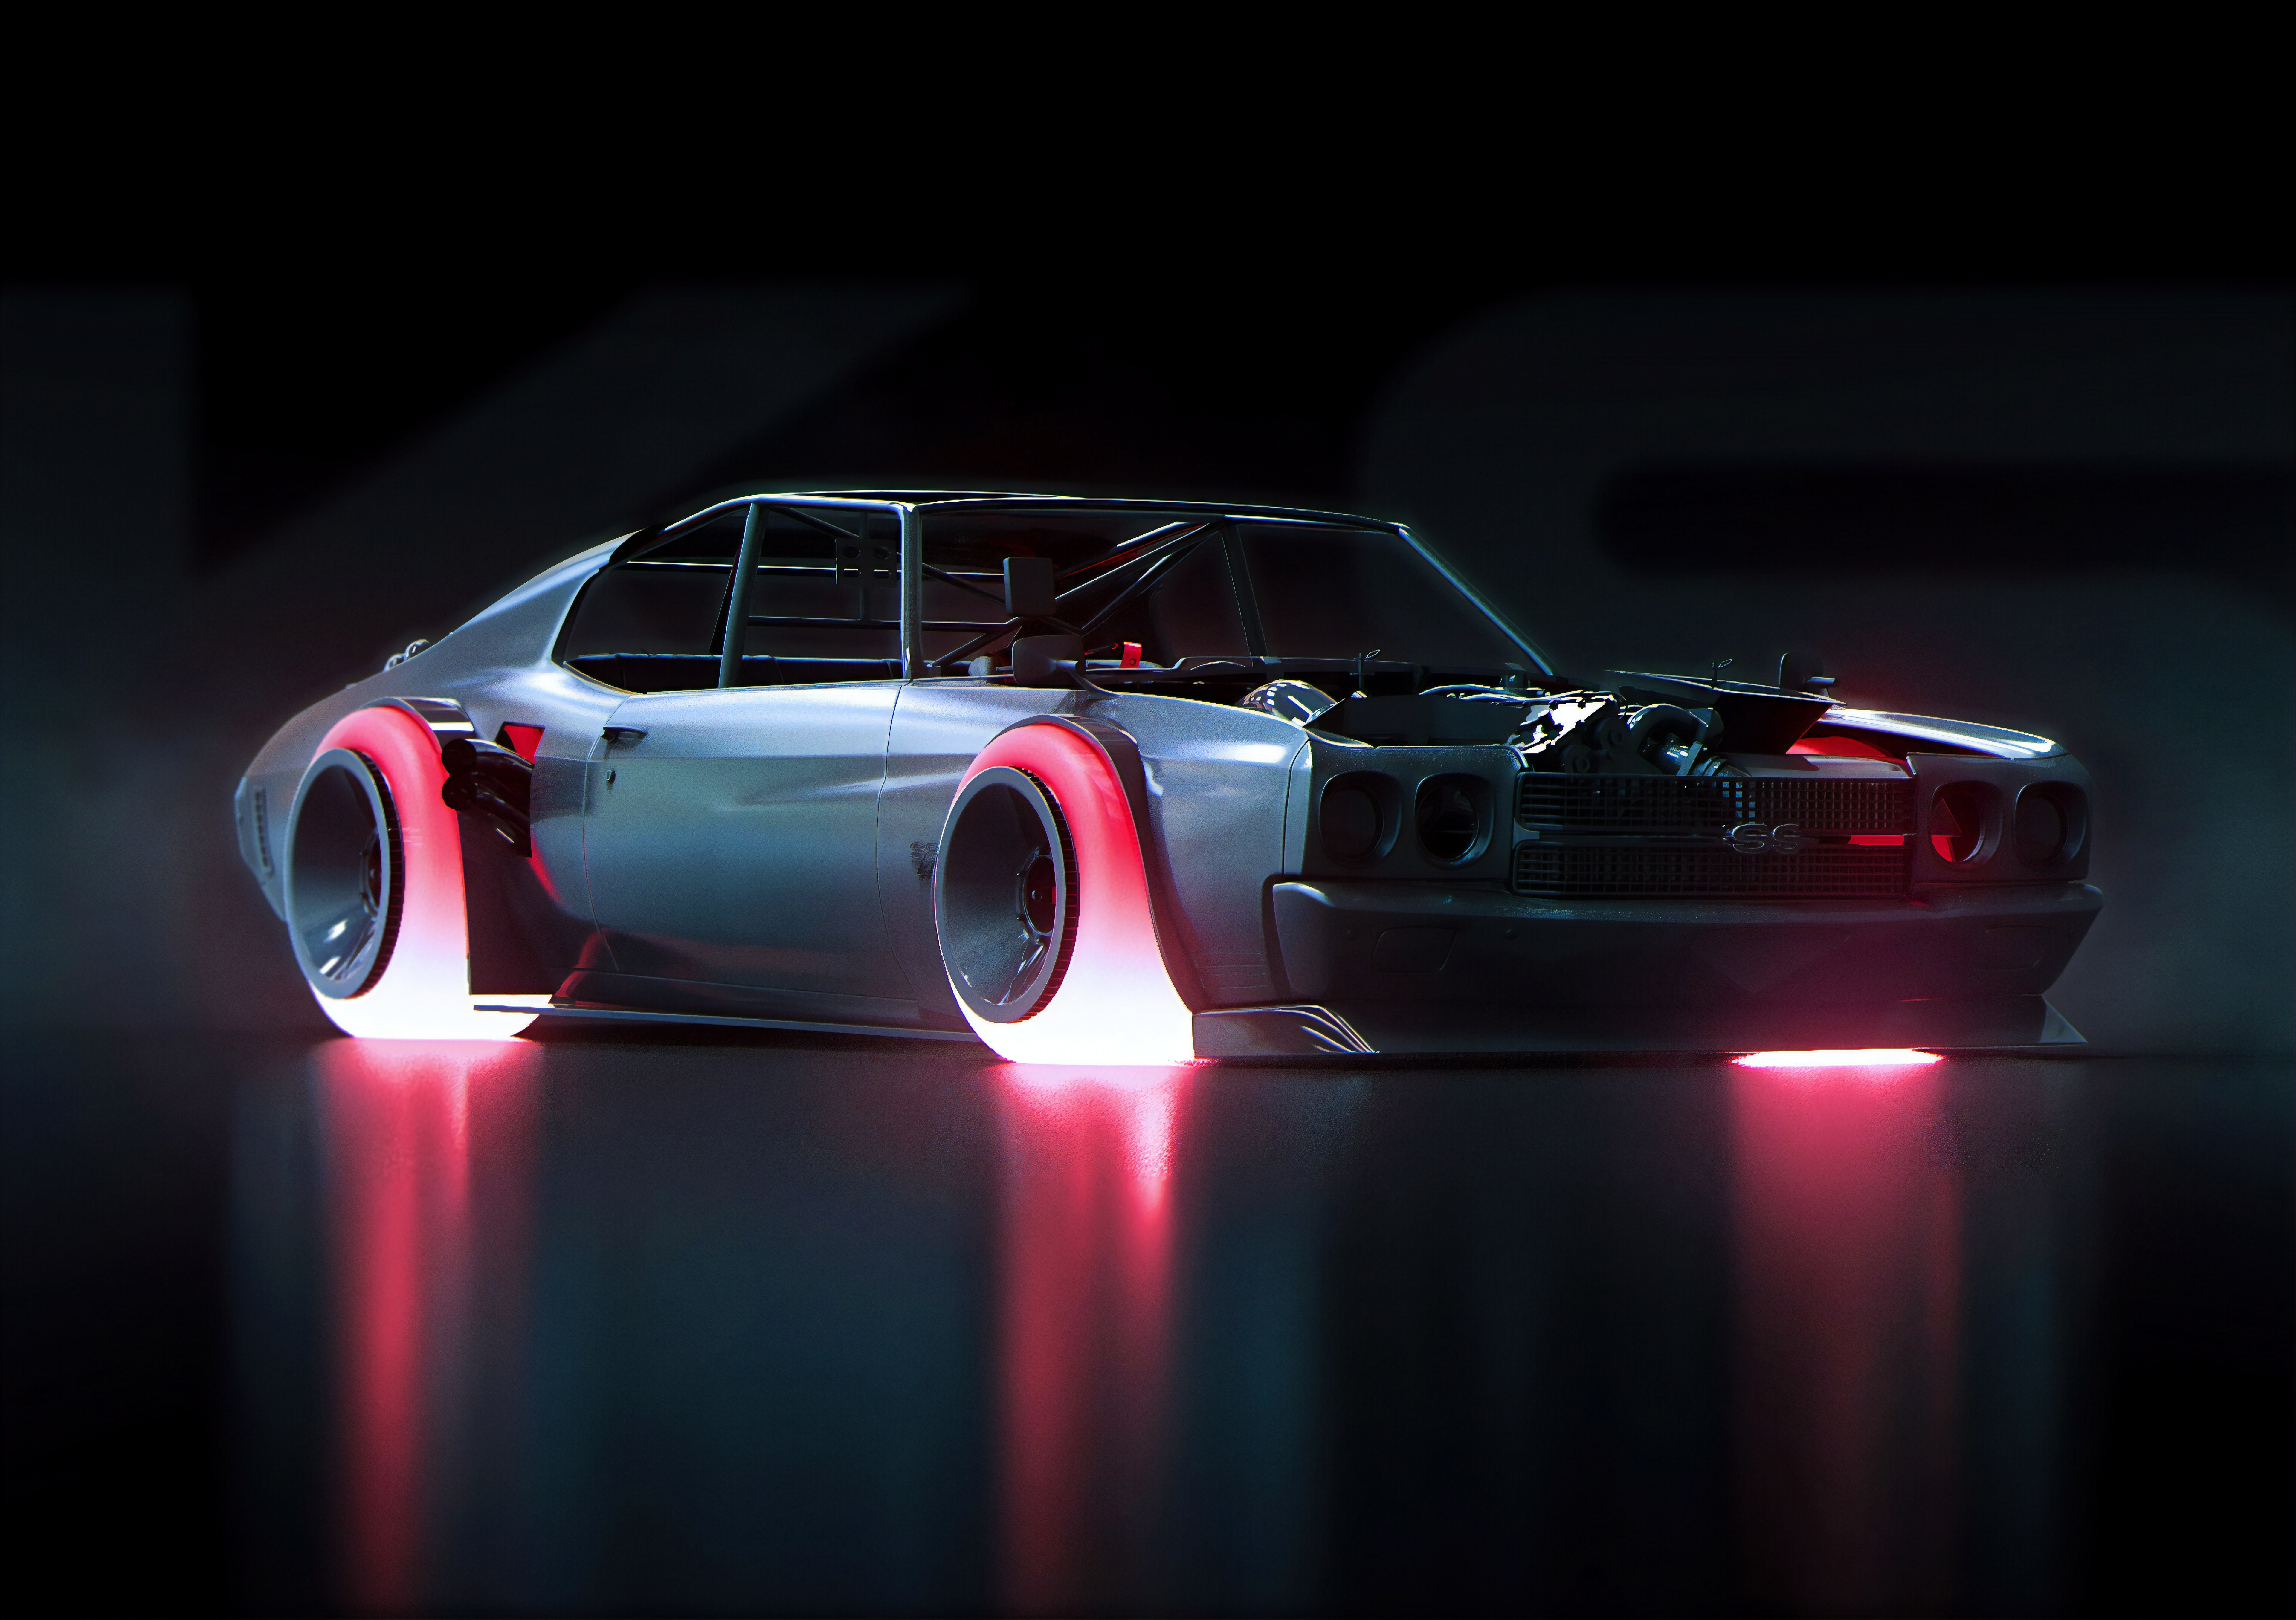
\includegraphics[width=0.4\textwidth]{7.png}
		\caption*{图6 减法器仿真电路图}
	\end{figure}
	\begin{table}[h]
	\centering
	\begin{tabular}{|c|c|c|c|}
		\hline
		输入信号$U_{i1}(V)$ & 0.2 & 0.2 & -0.2 \\
		\hline
		输入信号$U_{i2}(V)$ & -0.3 & 0.3 & -0.3 \\
		\hline
		计算值$U_O(V)$ & -4.99 & 1.01 & -0.987 \\
		\hline
		实际测量值$U_O(V)$ & \qquad & \qquad & \qquad \\
		\hline
	\end{tabular}
	\caption*{表3 减法器}
	\end{table}
	\section*{五、反相加法器}
	\begin{figure}[h]
		\centering
		
\includegraphics[width=0.4\textwidth]{8.png}
		\caption*{图6 反相加法器仿真电路图}
	\end{figure}
	\newpage
	\begin{table}[h]
	\centering
	\begin{tabular}{|c|c|c|c|}
		\hline
		输入信号$U_{i1}(V)$ & 1.0 & 1.5 & -0.2 \\
		\hline
		输入信号$U_{i2}(V)$ & 0.4 & -0.4 & 1.2 \\
		\hline
		计算值$U_O(V)$ & -1.4 & -1.1 & -0.997 \\
		\hline
		实际测量值$U_O(V)$ & \qquad & \qquad & \qquad \\
		\hline
	\end{tabular}
	\caption*{表4 反相加法器}
	\end{table}
	\section*{六、加减法器}
	\begin{figure}[h]
		\centering
		\includegraphics[width=0.4\textwidth]{9.png}
		\caption*{图6 加减法器仿真电路图}
	\end{figure}
	\begin{table}[h]
		\centering
		\begin{tabular}{|c|c|c|c|c|}
			\hline
			输入信号$U_{i1}(V)$ & $U_{i2}(V)$ & $U_{i3}(V)$ & 计算值$U_O(V)$ & 实际测量值$U_O(V)$ \\
			\hline
			0.4 & 0.8 & 0.4 & 11.1 & \qquad \\
			\hline
		\end{tabular}
		\caption*{表5 加减法器}
	\end{table}
\end{document}